\chapter{Day 8: Eigenface Synthesis and Project Kick-Off}

\section*{Schedule}
\begin{itemize}
\item 0900--1015		Debrief and Synthesis Activity on Eigenfaces
\item 1015--1030		Coffee Break
\item 1030--1115        Singular Value Decomposition --- Theoretical
\item 1115--1200        Singular Value Decomposition --- In action
\item 1200--1220        Review and Preview
\item 1220--1230        Survey
\end{itemize}

\section{Debrief and Synthesis Activity on Eigenfaces}

During the overnight assignment you implemented a facial recognition routine. For the first part of the morning, we want you to work with your table mates to think again about your method and implementation. 

\subsection{An Aside on Nearest Neighbor Classification}

One area where folks ran into trouble on the night assignment was the nearest neighbor approach to classification.  In nearest neighbor classification you classify a test point, $\mathbf{x_t}$ (think of representing this as a column vector containing a new piece of data like a face image of someone whose identity we don't know), by comparing it to a set of labeled training points $(\mathbf{x_1}, y_1), (\mathbf{x_2}, y_2), \ldots, (\mathbf{x_n}, y_n)$.  Each $y_i$ is the thing we are trying to predict (e.g., the identify of the person in a face image).  In nearest neighbor classification we check to see which of the $n$ training points is closest to the test point.  When we find the one that is closest, we predict the label for $\mathbf{x_t}$ to be the same as the label of the closest point in the training set.  To help get the idea across, here is a figure that shows all of your faces projected onto the first two principal components.  Also shown are the subject ids for each point.  You should be able to see from the figure that points with the same subject id tend to cluster together (i.e., are close together in facespace).  This is where the power of nearest neighbor classification comes from.

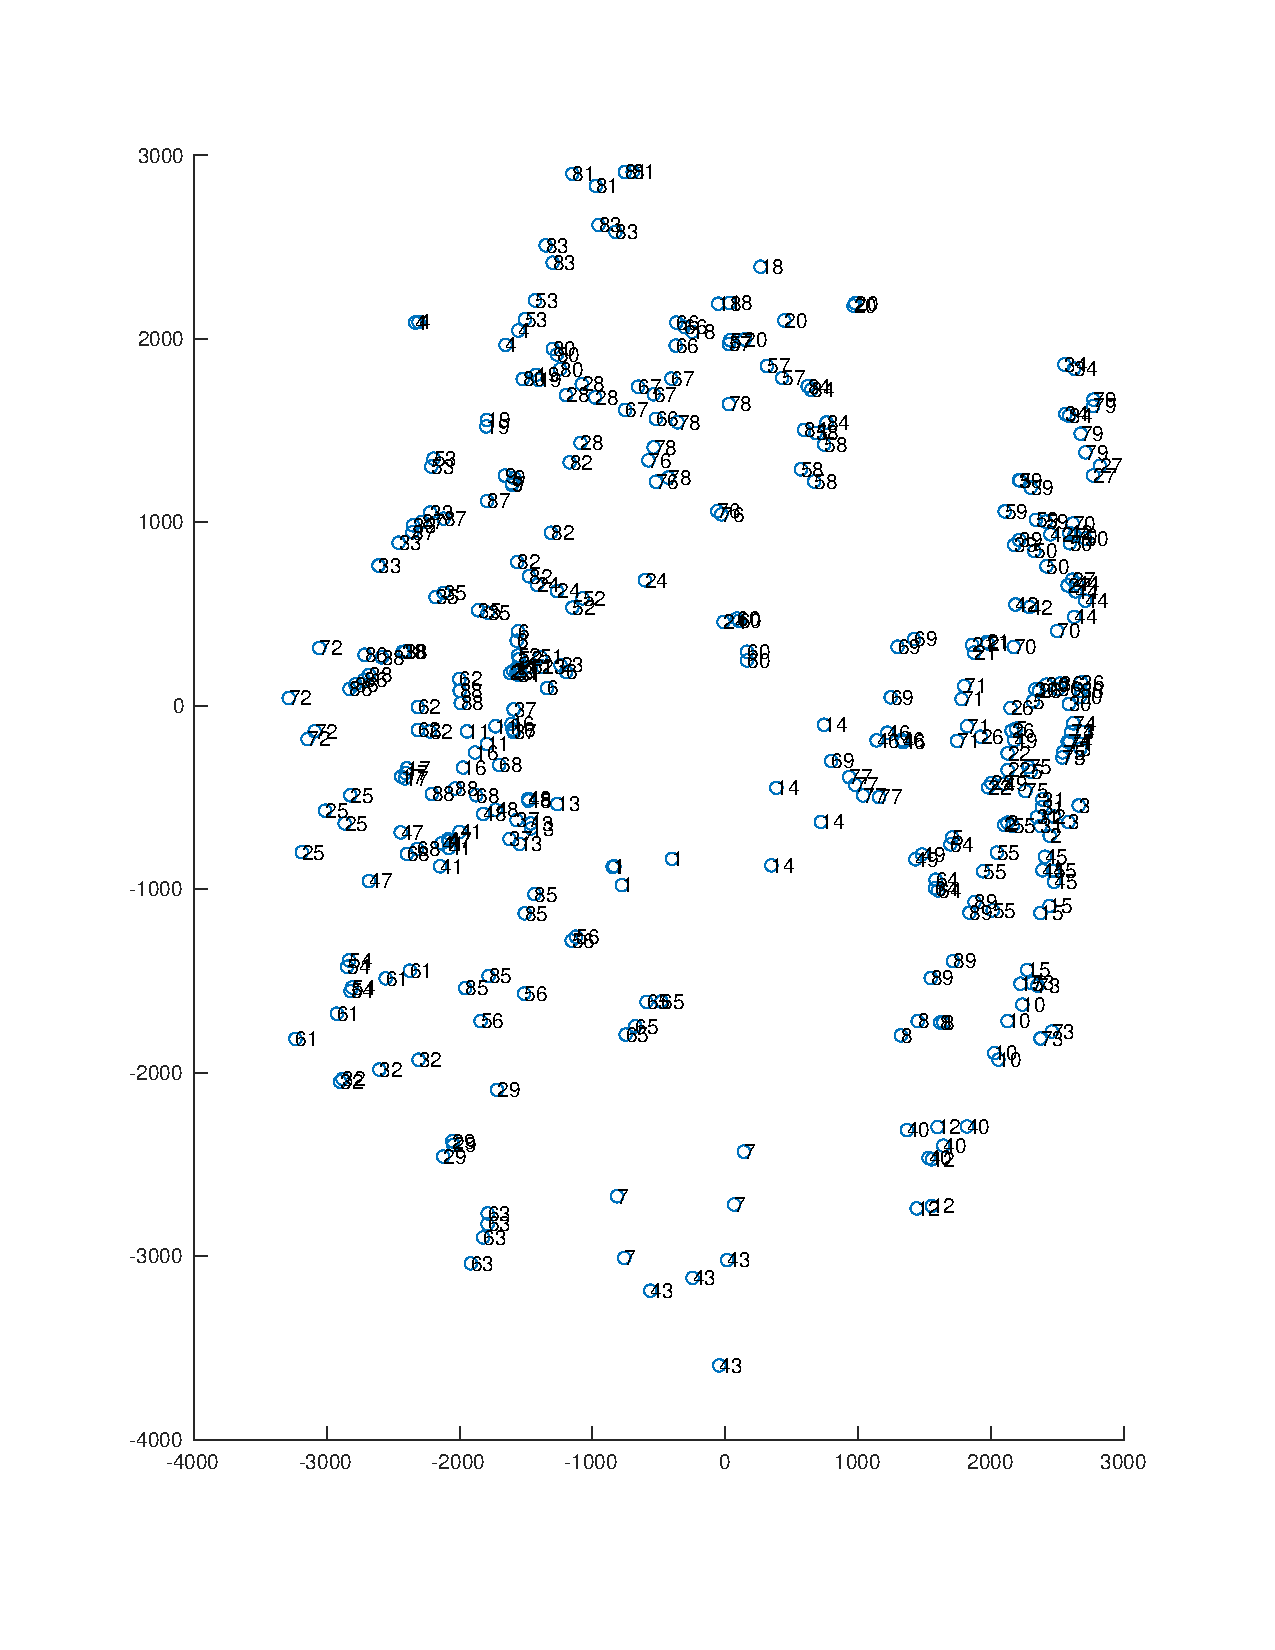
\includegraphics[width=\linewidth]{FacesDay8/figs/facespace}

\subsection{Eigenfaces Review [45 mins]}

We'd like you to take this opportunity to discuss with your table-mates the approach you took to facial recognition and the way you implemented it in MATLAB. The goal here is to think through the method at different levels from conceptual to code, resolving any confusion, and identifying whether any issues are primarily at the conceptual-level, the implementation-level, or the translation space in between. \textbf{We highly recommend that you set aside your existing code and focus on developing the approach with your table-mates.} Here are some questions to guide you:
\bi
\item Will you pre-process the data? If so, how?
\item How will you compute the Eigenfaces?
\item How will you decide how many Eigenfaces to include? Which Eigenfaces might you leave out?
\item How will you identify a face?
\item How will you measure the accuracy of your implementation?
\item How will you handle false positives?
\ei

\begin{prob}
\be
\item Sketch out on the board your conceptual approach to facial recognition---use words and diagrams here, and think of a set of key frames.
\item Sketch out on the board your mathematical approach to facial recognition---translate the key frames from your conceptual approach to mathematical expressions or equations.
\item Sketch out on the board your implementation approach to facial recognition---translate the key conceptual and mathematical ideas to MATLAB pseudo-code.
\ee
\end{prob}

\subsection{Eigenfaces Paper [45 mins]}

\textbf{This is on the next overnight assignment, but it would make sense to start this now if you have the time.}

Check out \href{https://drive.google.com/open?id=0B7LNBbaxYFujTkwxY1BZZEE2eWM}{\textit{Eigenfaces for Recognition}}, an early paper on eigenfaces, by M. Turk and A. Pentland. You have most of the tools to understand this paper, but the writing style might be unfamiliar (intense!). Spend 1 hour on this paper and then feel free to move on. The first 6 pages of this paper describe the use of eigenfaces in face recognition.

Check out other sources as well. Wikipedia is pretty useful for eigenfaces, and \href{https://drive.google.com/open?id=0B7LNBbaxYFujLUFfNThyT2JqNmc}{this} later paper talks about eigenfaces and an extension called Fisherfaces (not fish faces).

\begin{prob}
We are asking you read this paper for several reasons. We hope that it highlights and synthesizes all the material you've learned in this module. It will also give you practice reading a technical paper, which is a skill you'll continue to develop over your career.
\begin{enumerate}
    \item In what ways was your approach to implementing the eigenfaces algorithm similar or different from the authors' approach?
    \item In what ways did your understanding of the eigenfaces algorithm change after reading the paper?
    \item Were there places in the reading that you ``got stuck?'' If so, how did you address that?
    \item What questions do you have after reading the paper?
\end{enumerate}
\end{prob}

\section{Singular Value Decomposition (SVD) --- Theoretical}

We previously met the Eigenvalue Decomposition (EVD), which we used on square matrices. There is no EVD for rectangular matrices, but there does exist a generalization known as the Singular Value Decomposition, which is one of the most useful matrix decompositions in applied linear algebra. We will begin with some background concepts on singular values and singular vectors, and then explore them in the context of a user-movie rating data matrix. See the following webpage at the \href{http://www.ams.org/samplings/feature-column/fcarc-svd}{American Mathematical Society} for a good geometric discussion of the SVD.

\subsection{The Big Idea}

Rectangular matrices don't have eigenvalues and eigenvectors. However, they have a generalisation of these known as singular values and singular vectors. 

\bi
\item The singular values $\sigma_i$ and singular vectors $\u_i,\v_i$ of an $n \times m$ rectangular matrix $\A$ satisfy the definition
\begin{eqnarray}
\A \v_i &=& \sigma_i \u_i \label{righteq} \\
\A^T \u_i &=& \sigma_i \v_i \label{lefteq}
\end{eqnarray}
The singular vectors $\v_i$ are known as the \textbf{right singular vectors} and the singular vectors $\u_i$ are known as the \textbf{left singular vectors}. 

\item There are precisely $r=min(n,m)$ non-zero singular values. The singular vectors $\v_i$ are the eigenvectors of $\A^T \A$, and the singular vectors $\u_i$ are the eigenvectors of $\A \A^T$. The $r$ non-zero eigenvalues of $\A^T \A$ and $\A \A^T$ are $\sigma_i^2$.

\item The $n \times m$ matrix $\A$ has a \textit{singular value decomposition} (SVD) of the form
\begin{equation}
\A = \mathbf{U} \mathbf{\Sigma} \mathbf{V}^T
\label{svdeq}
\end{equation}
where $\mathbf{U}$ is an $n \times r$ orthogonal matrix whose columns are $\u_i$, $\mathbf{\Sigma}$ is an $r \times r$ diagonal matrix with $r$ non-zero entries $\sigma_i$, and $\mathbf{V}$ is an $m \times r$ orthogonal matrix whose columns are $\v_i$. Please note that this version of the SVD is called  the \textit{reduced} or \textit{economy} SVD - there is a more general form but this is the most useful in a practical setting.
\ei

\begin{prob}
\be
\item Read ``The Big Idea'' again!
\item Let's assume that $\A$ is a $3 \times 2$ matrix. What is the size of $\A^T$? What is the size of $\v_i$ and $\u_i$? What is the size of $\A^T \A$ and $\A \A^T$? How many eigenvalues will $\A^T \A$ have? How many eigenvalues will $\A \A^T$ have? What must be true about these eigenvalues according to ``The Big Idea''?
\item Show that $\sigma_i^2$ and $\v_i$ are the eigenvalues and eigenvectors of $\A^T \A$ by multiplying Equation (\ref{righteq}) by $\A^T$ and then using Equation (\ref{lefteq}) to simplify.
\item Show that $\sigma_i^2$ and $\u_i$ are the eigenvalues and eigenvectors of $\A \A^T$ by multiplying Equation (\ref{lefteq}) by $\A$ and then using Equation (\ref{righteq}) to simplify.
\item Take the transpose of Equation (\ref{lefteq}) and justify the use of the term \textbf{left singular vector} for $\u_i$.
\item Why is it valid to write
\[\A [\v_1 \ldots \v_r] = [\u_1 \ldots \u_r] \threebythree{\sigma_1}{}{}{}{\cdot}{}{}{}{\sigma_3}\]
and why does this imply Equation (\ref{svdeq})?
\item Why does Equation (\ref{svdeq}) imply that 
\begin{equation}
\A = \sigma_1 \u_1 \v_1^T + \sigma_2 \u_2 \v_2^T + \ldots + \sigma_r \u_r \v_r^T
\end{equation}
\item An $n \times m$ matrix has $nm$ data values. How many data values do you need to store $\sigma_1$, $\u_1$, and $\v_1$? What kind of compression ratio would you have if you only stored the first singular value and the first singular vectors?
\ee
\end{prob}

\section{Singular Value Decomposition (SVD) --- In Action}

We're going to be using a LiveScript notebook to go through an example of using SVD to analyze movie ratings.

You'll need to download both the dataset (movielens25m.mat) and the LiveScript (movieLens25m.mlx) before getting started.  We have included a PDF of the LiveScript in this document for your referene.

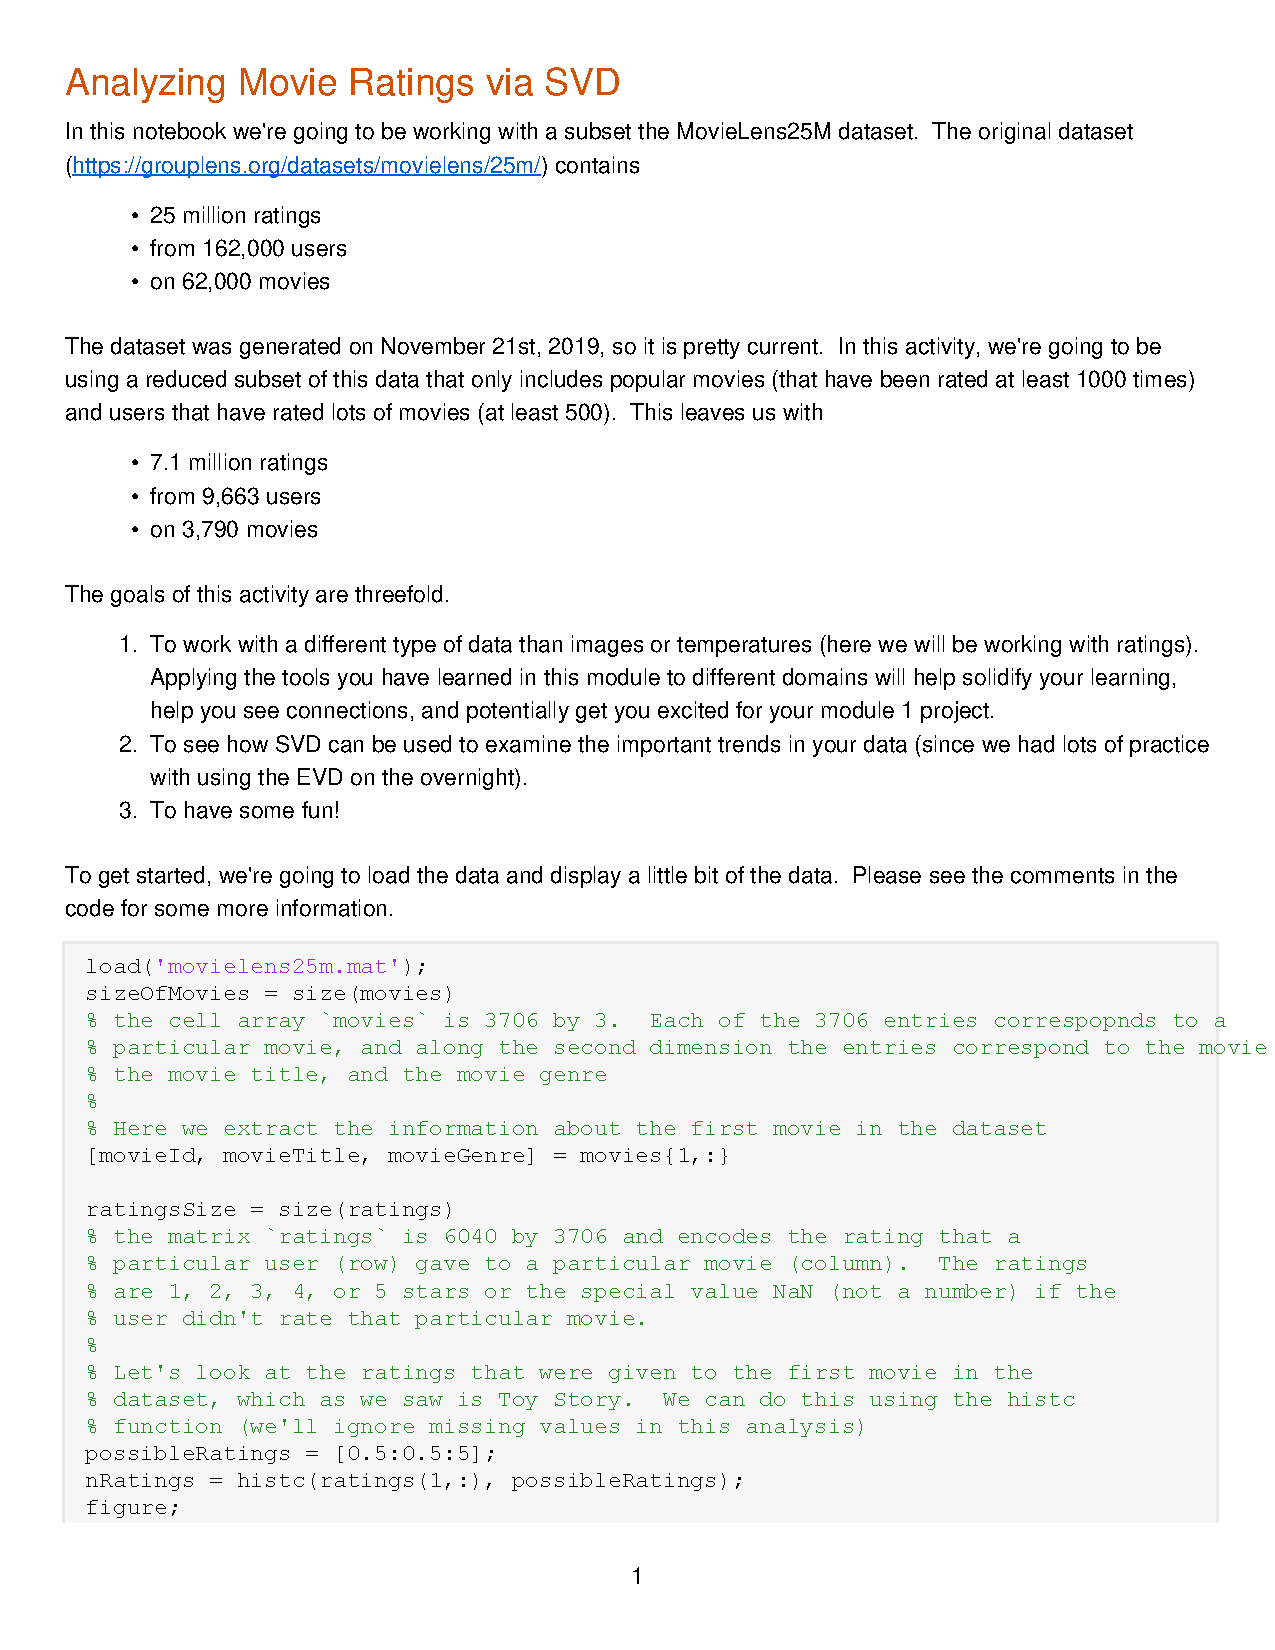
\includepdf[pages={1-}]{FacesDay8/movieLens25m.pdf}

\pagebreak
\shipoutAnswer

% Here is an example. Consider the rectangular matrix
% \[ \A = \begin{bmatrix} 1 & 2\\ 3 & 4 \\ 5 & 6 \\ 7 & 8 \end{bmatrix} \]
% Let's first form the matrix $\A^T \A$,
% \[ \A^T \A = \twobytwo{84}{100}{100}{120} \]
% The eigenvalues of $\A^T \A$ are $203.6071$ and $0.3929$ respectively. The singular values are the square roots of these, namely $\sigma_1 = 14.2691$ and $\sigma_2 = 0.6268$ respectively. The associated eigenvectors are
% \[\v_1 = \twobyone{0.6414}{0.7672} \]
% and
% \[\v_2 = \twobyone{-0.7672}{0.6414} \]
% so that the matrix $\mathbf{\Sigma}$ is
% \[ \mathbf{\Sigma} = \twobytwo{14.2691}{0}{0}{0.6268} \]
% and the matrix $\mathbf{V}$ is
% \[ \mathbf{V} = \twobytwo{0.6414}{-0.7672}{0.7672}{0.6414} \]
% To determine the $\mathbf{U}$ matrix, we now consider the matrix $\A \A^T$ (we will find another technique for determining $\mathbf{U}$ soon),
% \[ \A \A^T =
% \left[
% \begin{array}{cccc}
% 5&11&17&23\\
% 11&25&39&53\\
% 17&39&61&83\\
% 23&53&83&113
% \end{array}
% \right]
% \]
% The eigenvalues of $\A \A^T$ are $203.6071$, $0.3929$, $0$, and $0$.  The eigenvectors corresponding to the non-zero eigenvalues are
% \[ \u_1= \fourbyone{0.1525}{0.3499}{0.5474}{0.7448} \]
% and
% \[ \u_2 = \fourbyone{-0.8226}{-0.4214}{-0.0201}{0.3812} \]
% so that the $\mathbf{U}$ matrix is
% \[ \mathbf{U} = \begin{bmatrix} 0.1525 & -0.8226 \\ 0.3499 & -0.4214 \\ 0.5474 & -0.0201 \\ 0.7448 & 0.3812 \end{bmatrix} \]
% The original matrix $\A$ therefore has the SVD
% \[ \A = \begin{bmatrix} 0.1525 & -0.8226 \\ 0.3499 & -0.4214 \\ 0.5474 & -0.0201 \\ 0.7448 & 0.3812 \end{bmatrix} \twobytwo{14.2691}{0}{0}{0.6268}
% \twobytwo{0.6414}{-0.7672}{0.7672}{0.6414}^T \]

% \begin{prob}
% \begin{enumerate}
% \item Find the SVD of the following matrices by considering the eigenvalues and eigenvectors of $\A^T \A$ and $\A \A^T$. (You can use \texttt{eig} in MATLAB.)
% \begin{enumerate}
% \item \[ \threebytwo{1}{1}{0}{1}{-1}{1} \]
% \item \[ \begin{bmatrix}
% 3 & 2 & 2 \\ 2 & 3 & -2
% \end{bmatrix} \]
% \end{enumerate}
% \item Now use the \texttt{svd} command in MATLAB and check your work makes sense. You will need to use the "economy" option.

% \item Notice that the singular values and singular vectors satisfy the equations
% \begin{eqnarray*}
% \A \v_i &=& \sigma \u_i \\
% \A^T \u_i &=& \sigma_i \v_i
% \end{eqnarray*}
% Use this fact to confirm that $\v_i$ are the eigenvectors of $\A^T \A$, $\u_i$ are the eigenvectors of $\A \A^T$, and $\sigma_i^2$ are the non-zero eigenvalues of $\A^T \A$ and $\A \A^T$. 
% \end{enumerate}
% \end{prob}

% In data analysis, the economy SVD is very helpful in analyzing covariance matrices, because recall that if we have a data matrix with the mean subtracted out $\mathbf{A}$, the covariance matrix is $\mathbf{R} = \mathbf{A}^T\mathbf{A}$. E.g. if you have two variables $x$ and $y$ with means $\mu_x$ and $\mu_y$ respectively and define

%     \begin{align*}
% \mathbf{A} = \frac{1}{\sqrt{N}} \begin{pmatrix}
%     {x_1-\mu_x} & {y_1-\mu_y}\\
%   {x_2-\mu_x} &  {y_2-\mu_y}\\
%     {x_3-\mu_x} & {y_3-\mu_y}\\
%     \vdots & \vdots \\
%     x_N - \mu_x & y_N - \mu_y
%  \end{pmatrix}\,,
% \end{align*}

% We may only be interested in finding a few of the eigenvectors of $\mathbf{R}$,  in particular, we might only be interested in finding the eigenvectors corresponding to the non-zero eigenvalues of $\mathbf{R}$ (More on this later). Instead of computing all the eigenvectors, we could just compute a small number of them, which can be done much more quickly than computing all of them. This approach will become handy when we have more variables than we have data -- a situation you are bound to encounter in your project, and for which remembering this fact will be tremendously useful :).
% %LV end of insert content from D6

% %LV begin insert SVD content
% \section{SVD in Data Analysis}

% In data analysis, the economy SVD is very helpful in analyzing covariance matrices. Assume that we have a data matrix $\A$ with the mean subtracted out and normalized by the square-root of the number of data elements
%     \begin{align*}
% \mathbf{A} = \frac{1}{\sqrt{N}} \begin{pmatrix}
%     {x_1-\mu_x} & {y_1-\mu_y}\\
%   {x_2-\mu_x} &  {y_2-\mu_y}\\
%     {x_3-\mu_x} & {y_3-\mu_y}\\
%     \vdots & \vdots \\
%     x_N - \mu_x & y_N - \mu_y
%  \end{pmatrix}\,,
% \end{align*}
% where  $\mu_x$ and $\mu_y$ are the means of $x$ and $y$. The covariance matrix is then $\R = \A^T \A$.

% We may only be interested in finding a few of the eigenvectors of $\mathbf{R}$,  in particular, we might only be interested in finding the eigenvectors corresponding to the non-zero eigenvalues of $\mathbf{R}$ (More on this later). Instead of computing all the eigenvectors, we could just compute a small number of them, which can be done much more quickly than computing all of them. This approach will become handy when we have a lot more variables than we have data -- a situation you are bound to encounter in your project, and for which remembering this fact will be tremendously useful.  Keep this in mind as you work through the following review of SVD adapted from the work before break.
